\section{Højttalerdesign}
Højtalersystemet består som nævnt tidligere af højttalerenheder fra en defekt højtaler. Det er to diskantenheder (35 W/4 Ohm) og to bass/midrange (70 W/4 Ohm) enheder fra et gammel B\&O Beosound 8 system. 
\begin{figure}[H] 
	\center
		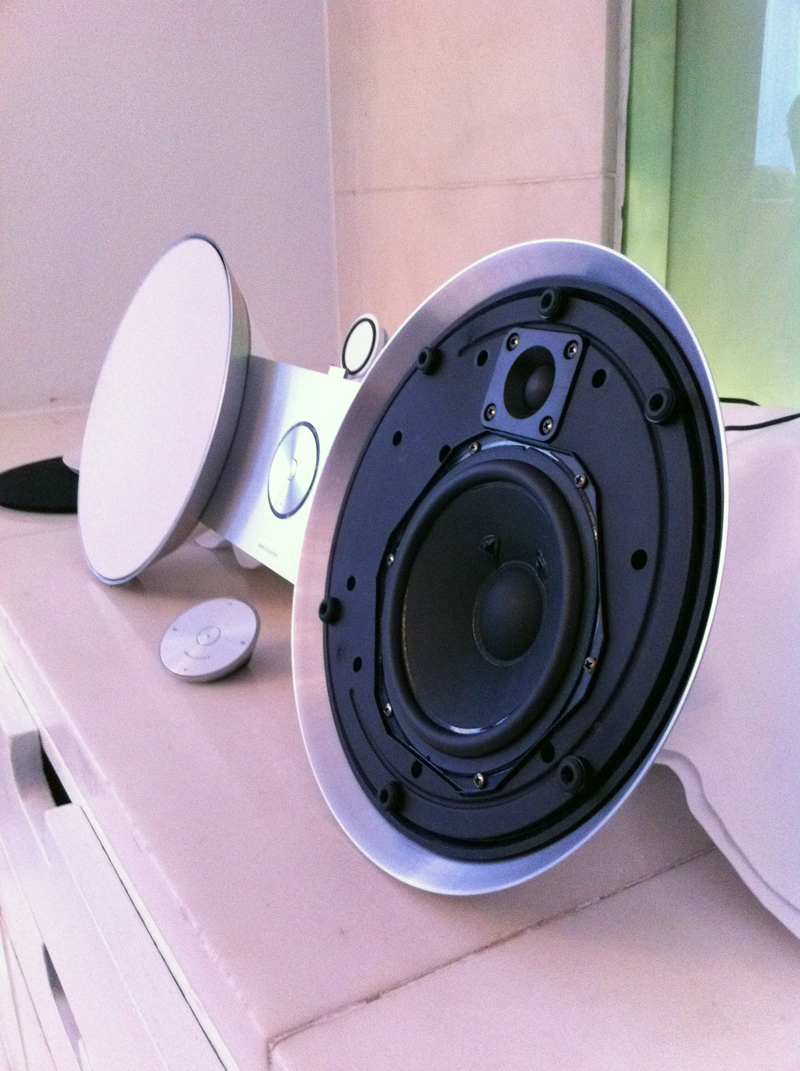
\includegraphics[width=.4\linewidth]{figur/bs8_enheder}\quad
		\caption{B\&O Beosound 8 enhederne som pille ud og bruges til festiavlanlægget}
		\label{fig:speakers}
\end{figure}

Da der ikke er så meget yderlig data på enhederne laves derfor et frekvenssweep (10 cm afstand) for at se hvordan enhederne frekvenskarakteristik ser ud. Dette gøres i det lyddøderum og resultatet kan ses i \autoref{fig:enheder}. Diskanten beskyttes med en $47\mu F$ kapacitor i serie inden enheden for at danne et highpass filter ved 846.57Hz som fjerner de laveste frekvenser for enheden.

\begin{figure}[H] 
	\center
		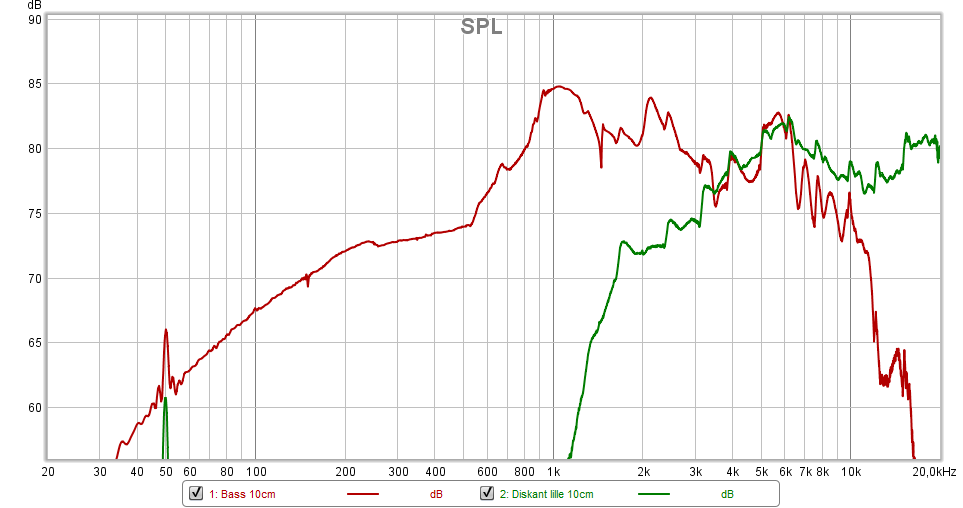
\includegraphics[width=.9\linewidth]{figur/Enheder-10cm}\quad
		\caption{Frekvenskarakteristik for enhederne 10cm afstand}
		\label{fig:enheder}
\end{figure}

Som det kan ses i \autoref{fig:enheder} har enhederne cirka samme følsomhed. Bassen ser ud til at fungere fint op til cirka 6-7 kHz men har et dyk ved 3-5kHz. Diskanten fungere også fint ned 1,7kHz, men aftager allerede ved omkring 5kHz. Derfor vil det i første omgang være ideelt at lave et delefilter ved cirka 4kHz, da begge enheder krydser hinanden der. De to peaks ved 50 Hz skyldes formentlig støj fra målecomputerens blæser eller diverse strømforsyninger tæt på mikrofonen.

Bassen har dog ikke ret meget forstærkning under 1kHz, hvilket i første omgang skyldes akustisk kortslutning \cite[side 24]{Elektroakustik}. Dette sker fordi enhederne ikke er i noget kabinet og der måles i 10cm afstand, hvilket tillader at bas enhedens bagside trykbølge har modsat fortegn af bas enhedens forside trykbølge, og dermed sænkes enhedens grænsefrekvens. Som det ser ud nu, virker enheden som sin egen baffel, idet det er en 5" enhed med en radius på cirka 6,35cm. Grænsefrekvensen kan findes ved tommelfingerregelen til forholdet mellem baffelareal og akustisk kortslutning givet ved: \cite[side 44]{Elektroakustik}

\begin{equation}
f_b \approx \frac{c} {4 b} 
\end{equation}

Her er $c$ lydens hastighed, $b$ er bafflens/enhedens radius i meter og $f_b$ er den grænsefrekvens hvor den akustiske kortslutning er uden betydning længere, hvis at måleafstanden er langt større end $b$. Med en radius på enheden 6,35cm giver dette en grænsefrekvens på ca. 1350Hz. Dette kan dog løses ved at sætte basenheden i et kabinet så grænsefrekvensen falder eller måle endnu tætter på membranen (fx 1cm = nærfelt) så det negative bidrag for bagsiden bliver ubetydeligt. 

\subsection{Kabinet}
Grundet den elektriske kortslutning af basenheden kræver projektet et kabinet, til dette er der købt et gammelt højtaler par med basrefleks i en genbrugsforretning til 50 kr. Kabinettet har vi tilpasset til at kunne montere de nye enheder i, hvilket løser problemet med akustisk kortslutning. Basrefleksen kan evt lukkes med, så det bliver til et lukket kabinet, hvilket resultatet af kan ses under Optimering.

Derudover har vi tilført æggebakke skum på indersiderne af kabinet for at dæmpe resonanser inde i kabinettet. Skummet bruges altså til absorbering/dæmpning af de stående bølger i kabinettet givet ved $ \frac{c}{2L} $, hvilket resultere i mere klarhed for det, der bliver afspillet på højtaleren.

Da diskant enheden i kabinetet har et større hul end den nye diskant, blev vi nød til at lave en holder til vores nye enhed. Dette blev lavet ved at 3-D printe en holder til diskantenhederne, som derefter blev monteret på kabinettet. 3-D printet skulle dog ikke tilføje en ny resonans frekvens, så derfor blev printet massivt. På figur \ref{fig:Sketchup} ses hvordan holderen er lavet i programmet SketchUp. De 4 huller bruges til at skrue holderen på kabinettet. 

\subsection{Delefilter}
Først beskyttes diskanten med en $47\mu F$ kapacitor i serie inden enheden for at danne et highpass filter ved 846.57Hz som fjerner de laveste frekvenser for enheden. Dette 1. ordens højpass filter gør, at diskanten under denne frevens bliver dæmpet med 6dB/oktav (20dB/dekade). 

Det egentlige delefilter også kaldet crossover laves på miniDSP'en med et 48dB/oktave Butterworth filter, som deler signalet ved 4kHz. Det er et meget stejlt filter, som også drejer fasen voldsomt, og man kunne godt argumentere for at bruge et lavere ordens filtre. Heldigvis kan dette ændres på 5 min, hvis det ønskes. Butterworth er valgt istedet for et Linkwitz–Riley filter, da højtaleren godt kunne bruge et lille boost ved delefrekvensen på 4kHz. Ved Butterworth giver det netop +3dB forstærkning ved delefrekvensen, da diskanten og bassen hver især kun er dæmpet 3dB ved denne frekvens, hvorimod et Linkwitz–Riley filter dæmper begge enheder 6dB ved delefrekvensen, så den resulterende forstærkning bliver 0db.  

Delefiltret for basenhederne kan ses herunder i \autoref{fig:delefilter_bass} og det tilsvarende delefilter for diskantenhederne kan ses herunder i \autoref{fig:delefilter_diskant}
\begin{figure}[H]
	\center
	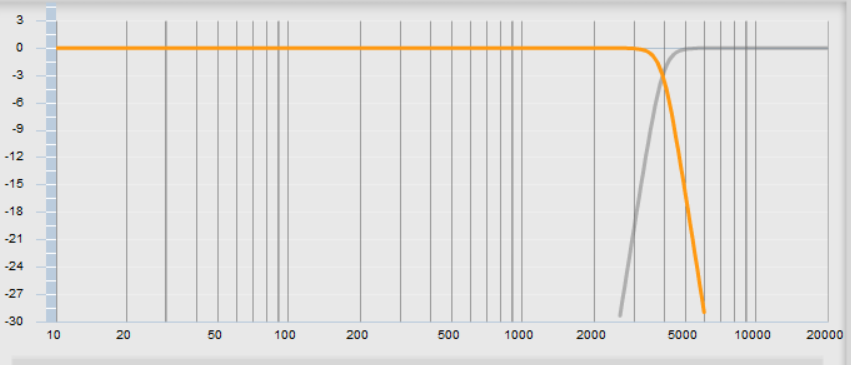
\includegraphics[width=0.9\textwidth]{figur/delefilter_bass}
	\caption{Frekvenskarakterstik for delefilter for bas kanalerne }
	\label{fig:delefilter_bass}
\end{figure}

\begin{figure}[H]
	\center
	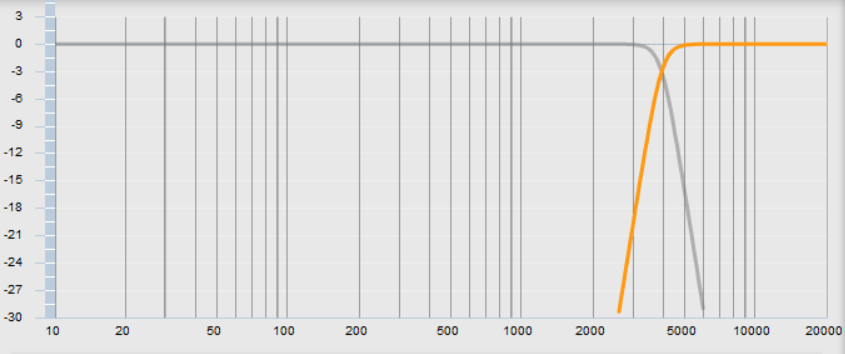
\includegraphics[width=0.9\textwidth]{figur/delefilter_diskant}
	\caption{Frekvenskarakterstik for delefilter for diskant kanalerne }
	\label{fig:delefilter_diskant}
\end{figure}

Som det kan ses i \autoref{fig:delefilter_bass} og  \autoref{fig:delefilter_diskant}, deler MiniDSP'en altså signalet ved den ønskede frekvens på 4kHZ, som netop gør at bassen ikke får nogle højfrekvente toner og ligeledes får diskanten ikke nogen lavfrekvente toner. Idet filtret er så stejlt og skarpt, som det er, så bidrager begge enheder med deres lydtryk næsten helt hen til grænsefrekvensen. Enhederne begynder altså ikke at runde så tidligt, som hvis det havde været fx et 12dB/oktav Butterworth filter.
 

